\documentclass[titlepage,12pt]{report}

\usepackage[utf8]{inputenc}
\usepackage[a4paper, total={6in, 8in},headheight=14pt]{geometry}
\usepackage{newtxtext,newtxmath}
\usepackage[scaled=1]{couriers}
\usepackage[spanish]{babel}
\usepackage{microtype}
\usepackage[bottom]{footmisc}
\usepackage{fancyhdr}
\usepackage{graphicx}
\usepackage{blindtext}
\usepackage{scrextend}
\usepackage{tocloft}
\usepackage{parskip}
\usepackage{multicol}
\usepackage{subcaption}
\usepackage{wrapfig}
\usepackage{multicol}
\usepackage{verbatimbox}
\usepackage[nottoc, notlot, notlof]{tocbibind}
\usepackage{listingsutf8}
\usepackage{url}
\usepackage[square,numbers]{natbib}
\usepackage{adjustbox}
\usepackage[makeroom]{cancel}
\usepackage[hidelinks]{hyperref}
\usepackage[Glenn]{fncychap}
\usepackage{lastpage}
\usepackage{fancyhdr}

\bibliographystyle{unsrtnat}

\pagestyle{fancy}
\fancyhf{}
\fancyhead[R]{\rightmark}
\fancyfoot[C]{\leftmark}
\fancyfoot[R]{\thepage}
\renewcommand{\footrulewidth}{0.6pt}% Line at the footer visible
\addto\captionscatalan{%
  \renewcommand\contentsname{Índice}%
}

\fancypagestyle{plain}{%
  \fancyhf{}%
  \fancyfoot[R]{\thepage}%
  \renewcommand{\headrulewidth}{0pt}% Line at the header invisible
  \renewcommand{\footrulewidth}{0.6pt}% Line at the footer visible
}


\renewcommand{\cftpartleader}{\cftdotfill{\cftdotsep}}%
\renewcommand{\cftsecleader}{\cftdotfill{\cftdotsep}}%
\renewcommand\familydefault{\sfdefault}

\usepackage{tikz}
\usetikzlibrary{shapes.geometric, arrows}

\newcommand{\Lagr}{\mathcal{L}}
\newcommand{\Xagr}{\mathcal{X}}

\setlength{\skip\footins}{1cm}

\makeatletter
% \patchcmd{<cmd>}{<search>}{<replace>}{<success>}{<failure>}
\patchcmd{\@makechapterhead}{\huge}{\large}{}{}% for \chapter
\patchcmd{\@makechapterhead}{\Huge}{\large}{}{}% for \chapter
\patchcmd{\@makeschapterhead}{\Huge}{\large}{}{}% for \chapter*
\makeatother


\begin{document}

\iftrue
\newcommand{\HRule}{\rule{\linewidth}{0.5mm}}

\thispagestyle{empty}

\begin{center}

{\large Universitat Politècnica de Catalunya}

\medskip
{\large Facultat d'Informàtica de Barcelona (FIB)}

\vfill
{\bfseries\Large Bachelor's Degree Project}

\vfill
\centerline{\mbox{
\includegraphics[width=60mm]{media/FIB_UPC.png}}}

\vfill
\vspace{5mm}

{\LARGE Jordi Gil González}

\vspace{15mm}

% Title in English according to the official assignment
{\LARGE\bfseries Analysis of the Path Tracing \\ rendering method on CPU and GPU}

\normalfont \small \sffamily{}

\vfill

Computer Science Department


\vfill

\begin{tabular}{rl}
Bachelor's Degree Project Director: & Chica Calaf, Antoni \\
\noalign{\vspace{2mm}}
Study programme: & Computer Science\\
\noalign{\vspace{2mm}}
Specialization: & Computer Graphics\\
\end{tabular}

\vfill

\large Academic Year 2019/2020

\large \today

\end{center}

\newpage
\tableofcontents*
\fi

\newpage

\chapter{Contextualización y alcance del proyecto}

\section{Introducción} \label{introduction}

En la actualidad, las imágenes generadas por ordenador están muy presentes tanto en el entorno profesional como en el lúdico. La creación de imágenes realistas mediante el uso de computadoras se ha convertido en una necesidad a la orden del día. Industrias como el cine o los videojuegos requieren de algoritmos capaces de reproducir el mundo real en un entorno virtual y, si siempre que se pueda, en el menor tiempo posible.

El estudio de métodos que permiten renderizar imágenes realistas no es nuevo. Entre principios y mediados de los años 70 comenzaron a publicarse los primeros artículos científicos en referencia a la simulación de la luz y el color sobre superficies modelos tridimensionales. Para poder entender como funcionan estos métodos debemos tener presente la representación de modelos 3D. 

Para representar un modelo 3D se utiliza una ''malla de polígonos'', popularmente conocida como \textit{Mesh} y generalmente estos polígonos suelen ser triángulos. Ésta consiste en un conjunto de vértices conectados por aristas formando caras. Para cada una de estas caras podemos definir un vector normal ortogonal a ésta. En la Figura \ref{dolphin} podemos apreciar un ejemplo de modelo 3D representado por una malla de triángulos.

\begin{figure}[H]
	\centering
	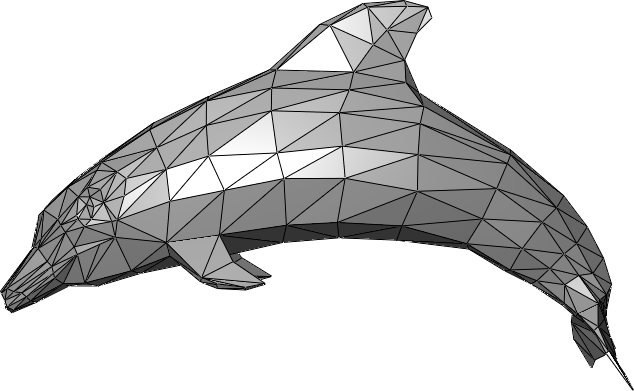
\includegraphics[scale=0.15]{media/Dolphin_triangle_mesh.png}
	\caption{Ejemplo de malla de triángulos. Fuente: Wikipedia}
	\label{dolphin}
\end{figure}

Volviendo a los métodos de cálculo de iluminación, el más simple de todos es el conocido como \textit{Flat Shading}. Para calcular el color de cada una de las caras de nuestra malla solamente tiene en cuenta un vértice de los que la conforman y la normal de ésta, aunque una malla compuesta por triángulos es común utilizar el centroide. El color se interpola para todos los vértices de la cara utilizando el color calculado al inicio dando así un resultado uniforme para toda la cara. Debido a no tener en cuenta las caras adyacentes esto produce resultados diferentes entre ellas. En la Figura \ref{flat:shading} podemos observar el efecto generado por este método. Podríamos pensar que añadir más vértices a nuestra malla los resultados mejorarían, pero no es una propuesta adecuada debido al mayor uso de memoria requerido y el problema no quedaría resuelto. Si hiciéramos \textit{zoom in} en el modelo, volveríamos a apreciar el efecto conocido como ''bandas de Mach'' \citep{Lotto1999}.

\begin{figure}[ht]
	\centering
	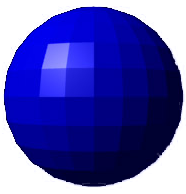
\includegraphics[scale=0.5]{media/Flat-shading-sample.png}
	\caption{Ejemplo de \textit{Flat Shading}. Fuente: Wikipedia}
	\label{flat:shading}
\end{figure}

En los métodos de sombreado suave (\textit{Smooth Shading}), el color cambia de pixel a pixel y no de cara a cara, resultando así en transiciones suaves entre las diferentes caras adyacentes.
En 1971 Henri Gouraud nos presenta en su artículo \textit{Continuous Shading of Curved Surfaces} \citep{Henri1971} el sombreado de Gouraud (\textit{Gouraud Shading}). Este método nos permite añadir mayor continuidad al sombreado respecto al método de \textit{Flat Shading}. El gran avance respecto al método presentado anteriormente es que no precisa de una malla de gran densidad para lograr simular una mayor continuidad. Para cada pixel se determina su intensidad por interpolación de las intensidades definidas en los vértices de cada polígono.

\begin{itemize}
	\item Para cada vértice se define una normal como promedio de las normales de los polígonos a los que pertenece dicho vértice.
	\item Mediante el uso de algún modelo de iluminación como, por ejemplo, el modelo de reflexión de Phong, se calcula la intensidad de cada vértice utilizando la normal obtenida en el punto anterior.
	\item Para cada pixel, se interpola la intensidad en los vértices para obtener la intensidad de éste.
\end{itemize} 

Como podemos observar en la Figura \ref{Gouraud:shading}, los resultados obtenidos respecto el método anterior son notablemente superiores, pero no acaba de representar de forma correcta los reflejos especulares. Éstos puede suponer un problema grave si se presentan en el centro de un polígono (cara) de gran tamaño.

\begin{figure}[ht]
	\centering
	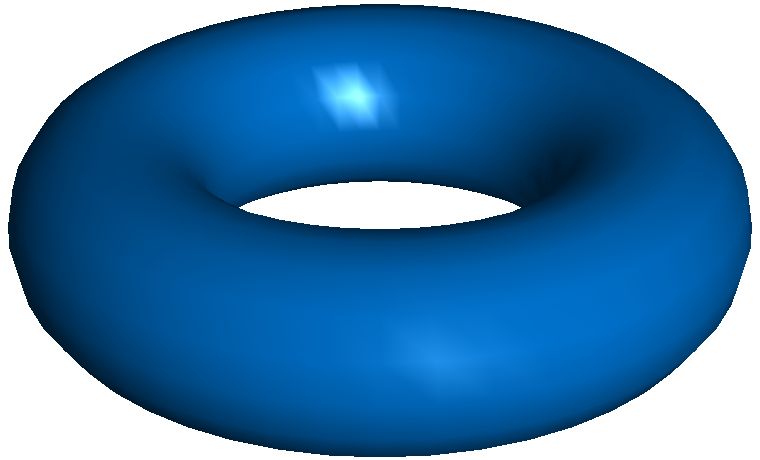
\includegraphics[scale=0.25]{media/Gouraudshading00.png}
	\caption{Ejemplo de \textit{Gouraud Shading}. Fuente: Wikipedia}
	\label{Gouraud:shading}
\end{figure}

Más tarde, Bui Tuong Phong en su tesis doctoral \citep{Phong1975} nos presentaba el sombreado de Phong. En el método presentado por Phong en vez de calcular la intensidad en el vértice, primero se define la normal de éste, se interpola y normaliza para cada pixel y es entonces cuando haciendo uso de algún modelo de iluminación se determina la intensidad final. El modelo resulta más costoso computacionalmente, debido a que el calculo se hace a nivel de fragmento (pixel) y no a nivel de vértice.

Phong menciona en su artículo publicado por la ACM \citep[p.~311]{Phong1975} que su objetivo no era simular la realidad, sino más bien añadir cierto grado de realismo:
\vspace{5mm}

\begin{mdframed}[hidealllines=true,backgroundcolor=gray!20] ''\textit{In trying to improve the quality of the synthetic images, we do not expect to be able to display the object exactly as it would appear in reality, with texture, overcast shadows, etc. We hope only to display an image that approximates the real object closely enough to provide a certain degree of realism.}'' 
\end{mdframed}

A pesar de que estos métodos supusieron, en lo concerniente al realismo, un avance, no pretenden simular la realidad. Además, éstos solamente tienen en cuenta la luz ambiente, difusa y especular. No tienen presente la iluminación indirecta de la escena, factor importante a la hora de crear imágenes que produzcan efectos realistas tales como, por ejemplo, reflejos.

No fue hasta los años 80 en que aparecieron los primeros métodos capaces de renderizar imágenes realistas. Turner Whitted nos presentaba en la sexta conferencia anual sobre \textit{Computer graphics and interactive techniques (SIGGRAPH)} el método de trazado de rayos, conocido popularmente por su nombre en inglés, \textit{Ray Tracing} \citep{Whitted1980}. Este método está basado en el algoritmo de \textit{Ray Casting}, presentado por \citep{Appel1968}, consistente en trazar rayos desde el observador, uno por pixel, para determinar cual es el objeto más cercano. Además, una vez el rayo impacta en una superficie, basándonos en las propiedades de los materiales definidos en el objeto y las propiedades de la luz, se calcula el color. Se puede hacer uso de \textit{texture maps} para simular efectos como sombras. 

En 1986, David Immel et al. y James T. Kajiya, investigadores de la Cornell University y del California Institute of Technology (Caltech) respectivamente, presentaban de forma conjunta, en la décima tercera conferencia anual sobre \textit{Computer graphics and interactive techniques (SIGGRAPH)}, la \textit{Rendering Equation} \citep{Kajiya1986, Immel1986}. Dicha ecuación integral trata de resumir en una sola fórmula como la luz interactúa cuando impacta con una superficie haciendo uso de funciones probabilísticas llamadas "función de distribución de la reflectividad bidireccional", (BRDF por sus siglas en inglés). Ésta también tiene presente el ángulo en el que incide el rayo, la cantidad de fotones que llegan, los fotones emitidos desde otros puntos de la escena (iluminación indirecta), etc.

Otros métodos que nos permiten generar imágenes realistas a partir de calcular aproximaciones de la RE son: \textit{Bidirectional Path Tracing} presentado por \citep{Lafortune1993}, \textit{Photon Mapping} formulado por \citep{Jensen1996} y \textit{Metropolis light Transport} introducido por \citep{Veach1997}.

\section{Contextualización}

\subsection{Contexto} \label{ref:contexto}

Durante los estudios del grado, son varias las asignaturas dedicadas a la computación gráfica. En estas asignaturas se nos presentan los métodos de renderización realistas. Pero más allá de la introducción teórica a éstos, nunca se llegan a poner en práctica. De aquí nace la idea de realizar el presente proyecto, poder profundizar más en el tema de renderización realistas y así crear un aplicación en función a lo aprendido. Se pondrán también en práctica otros aspectos de la informática vistas en otras asignaturas como, por ejemplo, la creación de aplicaciones paralelas tanto en CPU como en GPU.

Como hemos indicado en la sección anterior, la renderización de imágenes realistas es un área de gran interés en el campo de la computación gráfica. Uno de los principales objetivos de ésta es ser capaces de renderizar imágenes indistinguibles de las del mundo real como, por ejemplo, fotografías. Siguiendo estas coordenadas, poder reproducir el comportamiento de la luz en un entorno virtual supone una tarea una importancia capital. Es primordial tener presente la iluminación global de una escena para poder obtener un alto grado de realismo. La iluminación global de una escena se compone de: \begin{enumerate*}[label=\roman*)] \item iluminación directa \label{item:dl}, \item iluminación indirecta \label{item:il} \end{enumerate*}. En la Figura \ref{globalil} podemos apreciar una representación gráfica de ambos tipos de iluminación.

\begin{figure}[!ht]
	\centering
	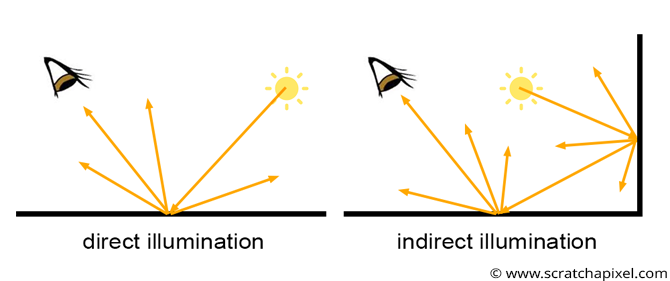
\includegraphics[scale=0.45]{media/shad2-globalillum3.png}
	\caption{Ejemplo de \textit{Iluminación directa e Iluminación indirecta}. Fuente: ScratchPixel}
	\label{globalil}
\end{figure}

\ref{item:dl} La iluminación directa es aquella que incide en un punto desde el foco de luz. \\
\ref{item:il} La iluminación indirecta es aquella que incide en un punto proveniente de la luz que rebota en otros puntos de la escena.

Recuperando lo expuesto en la introducción, el primer método capaz de renderizar imágenes realistas fue el \textit{Ray Tracing}, basado en la técnica de \textit{Ray Casting} de trazar rayos desde el observador a todos los pixeles de la imagen. La gran novedad respecto al algoritmo presentado por \citep{Appel1968} es la incorporación de la recursividad. En el \textit{Ray Tracing} se emite un rayo desde una cámara virtual hacia la escena para trazar el camino hasta los diferentes focos de luz de la escena. Cuando un rayo impacta contra un superficie puede generar tres tipos de rayos nuevos: \begin{enumerate*}[label=\roman*)] \item rayo de reflexión \label{ray:reflected}, \item rayo de refracción y \item rayo de sombra \end{enumerate*}. A partir de este punto, un nuevo rayo se proyecta hasta dar con las diferentes fuentes de luz de la escena. Al trazar los rayos nuevos somos capaces de conseguir efectos como reflejos, sombras, etc. debido a que para calcular el color estamos teniendo en cuenta como los demás objetos de la escena se afectan entre si. En caso de impactar con una superficie transparente, el rayo se proyecta a través de ésta para simular el efecto de refracción. Una gran desventaja de este método es la dependencia que éste tiene respecto a los polígonos de la escena; a más compleja es, más ineficiente será. 

A pesar de ofrecernos un alto grado de realismo al ser capaz de tratar con precisión efectos ópticos como la refracción, reflexión, los resultados obtenidos en una imagen renderizada mediante \textit{Ray Tracing} no son necesariamente foto-realistas. Se necesita hacer un postprocesado para simular efectos como sombras suaves (\textit{soft shwadows}, cáustica (\textit{caustics}), etc. Para conseguir renderizar imágenes foto-realistas, y por tanto efectos como cáusticas, debemos aproximar la RE, un buen ejemplo de ello es el método de \textit{Path Tracing} presentado por \citep{Kajiya1986}.

El algoritmo de \textit{Path Tracing} surge como mejora del \textit{Ray Tracing} con el objetivo de dar una solución a la RE mediante la integración de Monte Carlo. Es gracias a ésto que el algoritmo es capaz, de forma natural, representar efectos como \textit{Motion Blur}, \textit{Ambient Oclussion} e iluminación indirecta sin necesidad de posprocesado. A diferencia del \textit{Ray Tracing}, en el \textit{Path Tracing} cuando se emite un rayo desde la cámara virtual en vez de trazar el camino hasta los focos de luz de la escena, lo que hacemos es dejar que siga rebotando hasta golpear una fuente de luz o agotar un límite de profundidad en el número de rebotes que el rayo puede realizar. Pero la mayor diferencia respecto al método de Whitted es que en vez de tener en cuenta solamente el camino del rayo primigenio que emitimos, lanzamos decenas, cientos e incluso miles de rayos por pixel. Una característica importante del método de Kajiya es el muestreo aleatorio, esto significa que cuando un rayo impacta con una superficie éste genera uno nuevo en una dirección totalmente aleatoria. Una vez el rayo alcanza el límite de rebotes o es absorbido (por una fuente de luz) se calcula un valor en función de los objetos con los que rebotó y se añaden al promedio del pixel origen. Esta aleatoriedad provoca un resultado ruidoso que disminuye a medida que utilizamos más y más muestras por cada pixel.

\begin{figure}[!ht]
	\centering
	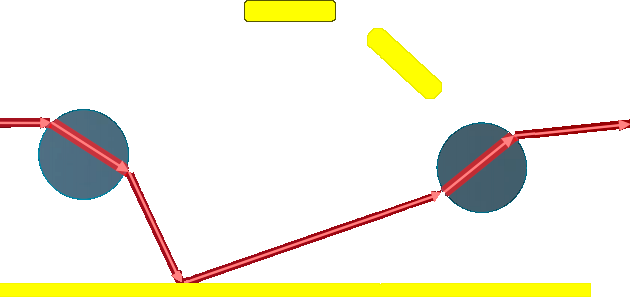
\includegraphics[scale=0.45]{media/lightPathRT.png}
	\caption{Trazado de rayo en \textit{Ray Tracing}.}
	\label{RT_traced}
\end{figure}

\begin{figure}[!ht]
	\centering
	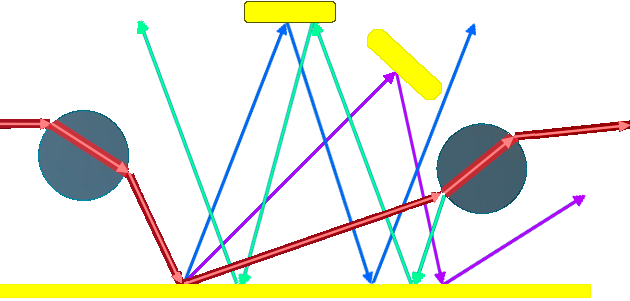
\includegraphics[scale=0.45]{media/lightPathPT.png}
	\caption{Trazado de rayo en \textit{Path Tracing}.}
	\label{PT_traced}
\end{figure}

En la Figura \ref{RT_traced} podemos observar aquello que comentamos en el párrafo anterior. En el \textit{Ray Tracing} el cálculo del color en un pixel solamente depende del trazado del rayo primario y como éste rebota por la escena hasta toparse con una fuente de luz. En cambio en la Figura \ref{PT_traced} se observa que a cada rebote, se generan múltiples rayos (en la imagen se ilustran un pequeña muestra). Esto ocurre porque cuando un rayo impacta contra una superficie difusa los fotones se dispersan en todas direcciones. Estos nuevos rayos nos permiten calcular la iluminación global para ofrecernos así un mayor realismo. 

El \textit{Path Tracing} es indiferente al número de polígonos presentes en la escena, la complejidad de la escena no afecta proporcionalmente al rendimiento del algoritmo. Como hemos mencionado anteriormente, en el primer método se traza un rayo por cada polígono de la escena, en cambio en el método de Kajiya el rayo se traza por pixel. Debido a que cada uno es independiente de los demás, tenemos un algoritmo con una alta capacidad de paralelismo. En consecuencia, podemos explotar la capacidad de concurrencia que nos proporcionan las CPUs y GPUs; y poder así calcular más de un pixel de la imagen al mismo tiempo.

\begin{figure}[H]
	\centering
	\begin{subfigure}{.3\textwidth}
		\centering
		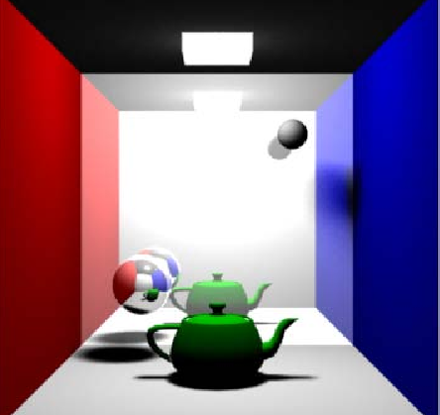
\includegraphics[width=.8\textwidth]{media/RayTracing.png}
		\caption{\textit{Ray Tracing}.}
		\label{RT}
	\end{subfigure}
	\begin{subfigure}{.3\textwidth}
		\centering
		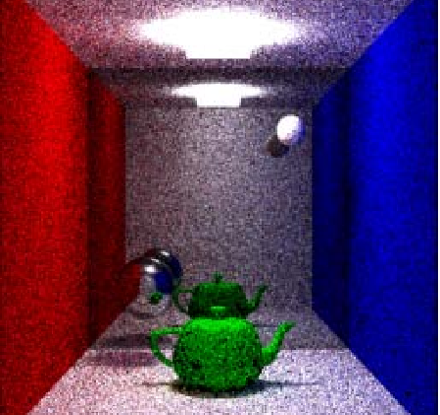
\includegraphics[width=.8\textwidth]{media/PathTracing.png}
		\caption{\textit{Path Tracing} con ruido.}
		\label{PTN}
	\end{subfigure}
	\begin{subfigure}{.3\textwidth}
		\centering
		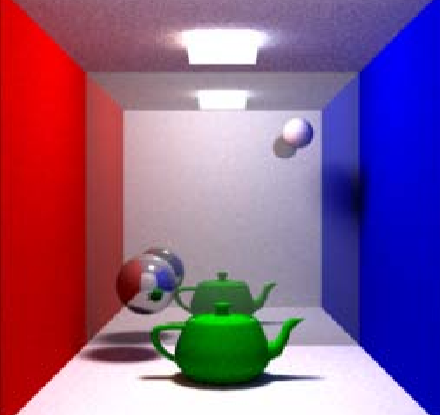
\includegraphics[width=.8\textwidth]{media/PathTracingMD.png}	
		\caption{\textit{Path Tracing} sin ruido.}
		\label{PT}
	\end{subfigure}
	\caption{Comparación \textit{Ray Tracing vs. Path Tracing}. Fuente: \citep{Cassagnabere2004}}
\end{figure}

Podemos apreciar como el \textit{Path Tracing}, Figura \ref{RT}, produce una sombras más suaves respecto al \textit{Ray Tracing}, Figura \ref{PT}. También se puede observar el efecto de ruido que provoca \textit{Path Tracing}, Figura \ref{PTN}, si pocas muestras por pixeles son utilizadas.

En el presente proyecto trataremos de crear un aplicación que implemente el método de \textit{Path Tracing} para generar imágenes de carácter realista. Dicha aplicación calculará cada pixel de la imagen final de forma secuencia, es decir, uno tras otro y nos servirá de base para crear una solución paralela haciendo uso de la GPU y otra haciendo uso de la CPU. El porque de realizar estas tres aplicaciones es para ser capaces de realizar un análisis del rendimiento que nuestro algoritmo obtiene explorando en profundidad la capacidad de concurrencia que nos ofrecen a día de hoy las CPUs y GPUs; y ver así que arquitectura nos ofrece mayor rendimiento.

Como base, partiremos de la implementación propuesta por Peter Shirley en su ''saga'' de libros sobre \textit{Ray Tracing} \citep{ShirleyRTA, ShirleyRTB, ShirleyRTC} para implementar nuestro \textit{Path Tracing}. La idea principal es desarrollar tres aplicaciones (una secuencia, una paralela en CPU y otra paralela en GPU) partiendo de la base que nos presenta Shirley, para poder hacer un análisis que como es el rendimiento de un \textit{Path Traing} explotando la capacidad de concurrencia de una CPU contra la de una GPU.

No solo nos centraremos en el apartado de renderizado, aunque se trata de la trama central de este proyecto, sino que estudiaremos también que técnicas de aceleración son comúnmente utilizadas para tratar de mejorar al máximo nuestro algoritmo. Es por ello que veremos también cual es la mejor manera de representar de forma interna la escena que queremos renderizar siguiendo la idea que nos presenta \citep{Karras2012} en su artículo.

La forma en que representemos nuestra escena tendrá un gran impacto a la hora de calcular el color de la imagen final. Como hemos comentado, la base del método es trazar rayos por la escena para calcular el color de cada pixel. Si nuestra representación de la escena consiste en almacenar todos los objetos en una estructura de datos de tipo lista o vector ordenados por orden de creación, a la hora de calcular un punto de la imagen en el peor caso estaremos recorriendo todo el conjunto de polígonos de la escena para determinar el color final. Tratar de renderizar una escena que, muy posiblemente, esté compuesta de millones de polígonos puede traducirse en horas y horas de procesado. Es por eso que haremos uso de una estructura de datos aceleradora que nos permita representar la escena de una forma más inteligente, para que a la hora de determinar si un rayo impacta o no un polígono se determine de la forma más rápida posible.

\subsection{Stakeholders}

En esta sección presentaremos cuales son los diferentes actores implicados en un proyecto.

\subsubsection{Desarrollador}

Este actor es el encargado de realizar la planificación del proyecto, búsqueda de información, documentación, desarrollo del software requerido, solución de posibles obstáculos y/o problemas que puedan aparecer a lo largo del desarrollo y realización y análisis de los experimentos. Debe trabajar de forma conjunta y coordinada con el director, y co-director y/o ponente si lo hay, y es la última persona encargada del cumplimiento de los términos establecidos.

\subsubsection{Director del proyecto}

Este actor es el encargado de guiar al desarrollador en caso de dificultades, así como del asesoramiento de posibles soluciones.

\subsubsection{Usuarios beneficiados}

Aunque este proyecto no tiene la intención de crear un producto, no quiere decir que no existan beneficiarios. Explorar diferentes vías de optimización haciendo uso de arquitecturas paralelas puede ser útil para investigadores y desarrolladores en el campo de la computación gráfica.

\section{Justificación}

Como bien hemos indicado en la sección anterior, partiremos de los libros presentados por Peter Shirley y el artículo sobre \textit{Bounding Volume Hierarchy} de Tero Karras para construir nuestras aplicaciones. En este trabajo lo que pretendemos es estudiar como podemos explotar al máximo las diferentes arquitecturas que tenemos en nuestra computadora (CPU y GPU) y ver en cual de ellas un método de renderizado de imágenes realistas se comporta de manera más eficiente. No podremos comparar nuestra solución aportada frente otras aplicaciones existentes que implementan también el método de \textit{Path Tracing} en GPU o CPU. En el ámbito de comparación de eficiencia en ciertas partes de la aplicación, como por ejemplo comprar el rendimiento del cálculo de la imagen final dada la representación de una escena, es difícil de comparar con aplicaciones que podrían ser similares debido que éstas están desarrolladas por expertos en la materia con una amplía experiencia y una serie de conocimientos que el autor del presente proyecto no tiene. Este conocimiento y experiencia les permite aplicar una serie de técnicas de optimización que pueden aumentar el rendimiento de forma notable. En el ámbito del realismo que podemos conseguir respecto el que consiguen otras aplicaciones también es complicado de comparar. La mayoría de aplicaciones que implementan un \textit{Path Tracing} no sólo implementan dicho método, sino que también implementan mucho más efectos, como por ejemplo \textit{subsurface scatering}. En el presente proyecto es imposible lograr una aplicación de características similares, primero por la falta de conocimiento o experiencia en el campo de renderización realista y segundo por el tiempo. Normalmente, un proyecto de estas dimensiones involucran a varios expertos en la materia y se disponen de más tiempo de realización. Un ejemplo de aplicación profesional es RenderMan de Pixar Animation Studios \citep{Christensen2018}.

Por esto mismo, en el presente proyecto realizaremos tres versiones del mismo algoritmo: \begin{enumerate*}[label=\roman*)] \item versión secuencial, \item versión paralela en CPU y \item versión paralela en GPU \end{enumerate*}. De esta forma podremos hacer una comparativa de que arquitectura nos brinda una mayor ventaja para nuestra implementación.

En la actualidad son muchas las librerías orientadas a la programación en GPU. Tenemos librerías como \texttt{OpenCL} y \texttt{OpenACC}, que nos permiten una mayor portabilidad entre tarjetas gráficas de distintos fabricantes como por ejemplo \texttt{AMD} y \texttt{NVIDIA}. Pero para este proyecto hemos decidido escoger el entorno de \texttt{CUDA} desarrollado por \texttt{NVIDIA} específicamente para sus tarjetas gráficas y aceleradores. Decidimos usar esta API debido a que se trata de software propietario, mejor optimizado para las tarjetas de dicha empresa como bien nos indican \citep{Karimi2010} y \citep{Fang2011} respectivamente en sus artículos científicos, las cuales utilizaremos en este proyecto.

Es posible que, citadas tarjetas/aceleradores \texttt{NVIDIA} y, teniendo presente que el proyecto está enfocado al tema de renderizado de gráficos realistas, al lector del presente Trabajo de Fin de Grado le venga a la mente la nueva gama de tarjetas RTX diseñadas por \texttt{NVIDIA}. En un inicio se planteó guiar el proyecto hacia el uso de tarjetas con tecnología RTX debido a que éstas han sido diseñadas específicamente para el uso de \textit{Ray Tracing} en tiempo real. Pero esta idea fue descartada en seguida debido al elevado precio de éstas. El rango de precios de las tarjetas de esta gama oscila entre los 350€ en los modelos más económicos, hasta los varios miles de euros en modelos destinados a entornos profesionales. Finalmente, aunque el autor de dicho trabajo adquirió una tarjeta gráfica NVIDIA RTX 280 Super con 8Gb de memoria, se decidió no guiar el proyecto a utilizarla de forma exclusiva, estudiando y poniendo en práctica las nuevas mejoras que ésta ofrece (RT Cores, Tensor Cores, Mesh Shaders, etc.), frente a otras tarjetas de gamas inferiores que no incluyen, debido al corto plazo de tiempo para el desarrollo. Es por eso que esta tarjeta gráfica será usada para testar nuestra aplicación, pero no en un sentido exclusivo. Enfocar el trabajo a explorar en profundidad las nuevas características introducidas no fue posible, hubiera significado reestructurar todo el proyecto desde cero. Esto hubiera supuesto una gran perdida del tiempo invertido en adquirir los conocimientos necesarios para realizar el presente proyecto, es por eso que no se decidió enfocar el trabajo en el gran potencial que nos brinda la tecnología RTX. Eso no quiere decir que no podamos utilizarla. Al ser una tarjeta gráfica de gama alta, el número de cores que tiene respecto a la GTX1050 (gama media) nos permitirá analizar cuan mejor es y si merece o no la pena, en relación coste-potencia, su uso en aplicaciones de este tipo.

Como hemos comentado al inicio de esta sección, \texttt{CUDA} es un API que está muy bien optimizada para hardware de \texttt{NVIDIA}. Esto nos da un punto a favor debido a que la aplicación que vamos a desarrollar será probada en diferentes entornos que utilizan la tecnología de NVIDIA:

\begin{enumerate}
	\item Computador portátil - Lenovo Legion Y520 con Nvidia GTX1050 Mobile - 4GB.
	\item Computador personal - Nvidia RTX 2080 Super - 8Gb.
	\item Cluster docencia BOADA - 4 GPUs Nvidia Tesla K40c.
\end{enumerate}

Al usar tarjetas en entornos diferentes podremos analizar como nuestra aplicación responde en cada uno de ellos y estudiar así cómo es el rendimiento cuando utilizamos varias tarjetas pensadas para un entorno de investigación/profesional, en contraposición con otras dos pensadas para un uso más cotidiano. También podremos ver como es el rendimiento en una tarjeta gráfica de gama media (Nvidia GTX1050 Mobile) y una de gama alta (Nvidia RTX 2080 Super); y hacer así una comparativa entre ellas.

\section{Alcance del proyecto}

Para solucionar el problema presentado en nuestro proyecto necesitamos una aplicación que sea capaz de renderizar imágenes realistas. Como hemos comentado unas secciones más atrás, en \citep{ShirleyRTA, ShirleyRTB, ShirleyRTC} se nos presentan las bases para crear un \textit{Ray Tracing}. A partir de esta base extenderemos nuestra aplicación a una versión paralela haciendo uso de la CPU y otra haciendo uso de la GPU.

También, como hemos comentado en la sección sobre el contexto, el uso de estructuras de datos aceleradoras es un factor importante en este tipo de aplicaciones y se llevan estudiando durante muchos años (p.e. \citep{Rubin1980}) por parte de la comunidad científica. En este proyecto haremos uso de la \textit{Bounding Volume Hierarchy}, que se trata de una estructura de tipo árbol, ya sea binario o n-aria, en el cual cada hoja representa la caja delimitadora (\textit{Bounding Box}) de cada primitiva de la escena; y cada nodo intermedio representa la caja delimitadora de sus hijos. De este modo, estamos representando la escena como un conjunto de cajas que nos permitirá saber de forma eficiente si un rayo impacta o no con un polígono y con cual de todos los que componen la escena.

Existen muchas formas de construir un BVH, en nuestro caso nos hemos decantado por la versión presentada por \citep{Karras2012, Karras2013}. La forma en la que construimos el árbol nos permite explotar al máximo la concurrencia que nos proporciona la CPU y la GPU ya que es posible construir cada nodo del árbol de forma independiente.

\begin{figure}[ht]
	\centering
	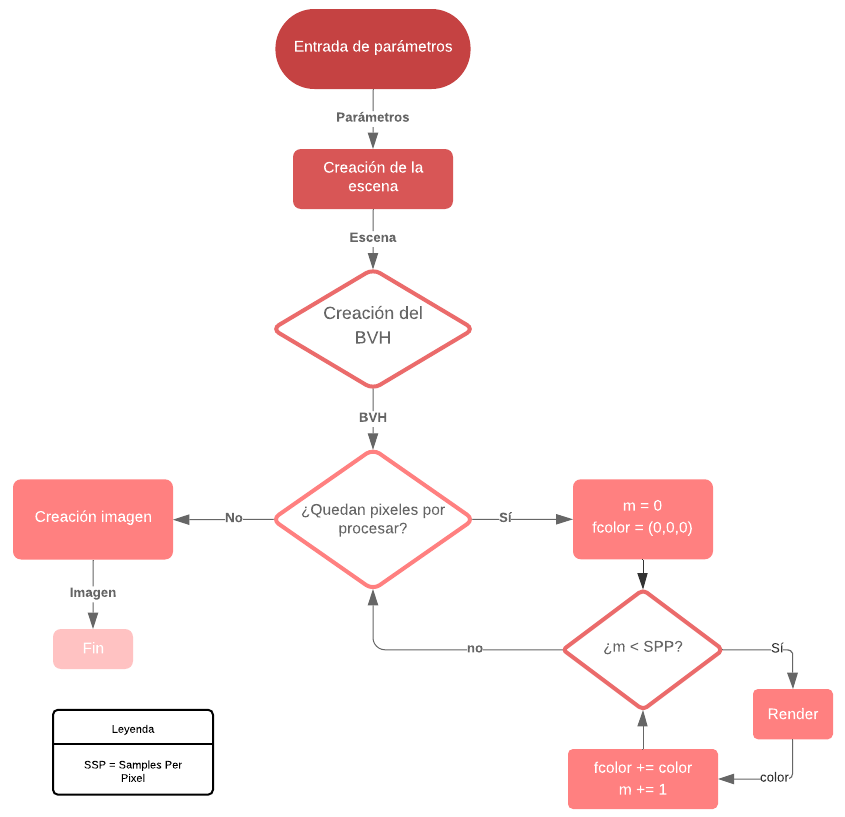
\includegraphics[scale=0.35]{media/Esquema.png}
	\caption{Esquema aplicación.}
	\label{Esquema}
\end{figure}

En la Figura \ref{Esquema} podemos observar un esquema, a grandes trazos, de cual comportamiento es el comportamiento de nuestra aplicación.

\subsection{Objetivos}

\subsubsection{Objetivos principales}

Son varios los objetivos principales que nos proponemos en este proyecto. El primero se trata de desarrollar tres aplicaciones (secuencial, paralela en CPU y paralela en GPU) que dada una escena la renderice mediante el método de \textit{Path Tracing} y analizar el rendimiento que éste nos ofrece entre las diferentes versiones con la intención de analizar que arquitectura nos brinda una mayor rendimiento en este tipo de aplicaciones.

Un segundo objetivo principal que nos proponemos en nuestro proyecto es estudiar y poner en práctica cuales son las mejores prácticas en la gestión de memoria en una aplicación paralela se refiere. Lo identificamos como un objetivo principal por que una mala gestión de ésta puede suponer un gran obstáculo en el desarrollo del proyecto.

\subsubsection{Objetivos secundarios}

Como objetivos secundarios, pero no menos importantes, tenemos:

\begin{enumerate}
	\item Implementar de forma eficiente el método presentado por P. Shirley y T. Karras.
	\item Buscar información sobre técnicas de optimización en el cálculo de intersección rayo-objeto.
	\item Implementar de forma eficiente los cálculos de intersección rayo-objeto.
	\item \label{3D} Extender la aplicación para renderizar modelos 3D.
	\item \label{GLUT} Creación de una aplicación interactiva.
\end{enumerate}

Los objetivos secundarios \ref{3D} y \ref{GLUT} se realizarán en función del tiempo restante para la finalización del proyecto.

\subsection{Obstáculos y riesgos del proyecto}

Los temas principales en los que se centra el presente proyecto han sido muy estudiados por parte de la comunidad científica. No obstante, esto no implica que el desarrollo de éste sea una tarea sencilla, pues son muchos los problemas u obstáculos a los cuales podemos enfrentarnos.

\subsubsection{Programa principal}

Como bien hemos comentado en la sección de objetivos, la gestión de memoria es un factor muy importante. Una mala gestión de ésta puede provocar errores que no permitan el correcto funcionamiento de la aplicación.

\subsubsection{Algoritmo utilizado}

El algoritmo utilizado calcula el color a partir de la intersección de los rayos emitidos desde la cámara a los diferentes pixeles de la escena. Al tratarse operaciones que se llevarán a cabo miles de millones de veces en la creación de una imagen, tener una mala implementación de éstas puede afectar al rendimiento de nuestra aplicación de forma negativa.

\section{Metodología y rigor}

En esta sección veremos el conjunto de herramientas que se usarán a lo largo del desarrollo del presente proyecto. Para poder llevar un buen desarrollo de éste nos organizaremos de la siguiente forma: \begin{enumerate*}[label=\roman*)] \item Reuniones cada 15 días con el director del presente proyecto para comentar el estado de éste, resultados obtenidos, carencias, objetivos cumplidos y no cumplidos y acordar los siguientes pasos a realizar. \item Reuniones semanales de cara a la fase final del desarrollo. \end{enumerate*}

\subsection{Metodología}

La metodología de trabajo que se seguirá en el presente proyecto es la conocida como \textit{agile}. Esta metodología se caracteriza por se iterativa. Es decir, en cada iteración hay una serie de tareas y cuando se finalizan estas se inicia una nueva iteración, conocidas como \textit{sprint}. En nuestro proyecto cada iteración del ciclo de vida corresponderá con el inicio de una reunión con el director del proyecto hasta el inicio de la siguiente vista. En cada reunión se especificará una serie de objetivos, que deberán cumplirse de cara a la siguiente vista y en la que se evaluarán cuales han sido cumplidos y cuales no. En la Figura \ref{agile} podemos observar un esquema representativo del funcionamiento de esta metodología.

\begin{figure}[ht]
	\centering
	
\includegraphics[scale=0.25]{media/agile.png}
	\caption{Esquema metodología ágil. Fuente: OpenWebinars}
	\label{agile}
\end{figure}

\subsection{Herramientas de desarrollo}

El desarrollo de nuestra aplicación se llevará a cabo en C++ haciendo uso de las librerías \texttt{OpenMP} y \texttt{CUDA}. 

\texttt{OpenMP} es una API diseñada para añadir concurrencia a programas escritos en \texttt{C}, \texttt{C++} y \texttt{Fortran}. La principal ventaja de usar esta API, en contra de otras de características similares, es que nos permite escribir un código portable entre diferentes sistemas operativos como podría ser Linux, Windows o MAC y nos permite crear de forma sencilla aplicaciones paralelas haciendo uso de la CPU.

\texttt{CUDA} es una plataforma de computación paralela y una API desarrollada por \texttt{NVIDIA} que nos permite acceder al conjunto de instrucciones y elementos de cómputo de las tarjetas gráficas y aceleradores de \texttt{NVIDIA} para poder crear aplicaciones paralelas haciendo uso de la GPU.

\subsection{Herramientas de seguimiento}

Por tal de llevar a cabo un buen seguimiento del desarrollo del presente proyecto se hará uso de \texttt{git}. Esta herramienta nos permite llevar un control de versiones que nos permitirá consultar versiones anteriores de nuestro código en caso de ser necesario.

\chapter{Planificación temporal}

\section{Planificación y programación}

Este capítulo trata la planificación del proyecto y describe las tareas realizadas, a través de un plan de acción, para cumplir los plazos relativos a la entrega del proyecto. Veremos también los recursos utilizados y se tendrán en cuenta los posibles obstáculos que puedan modificar la planificación.

El proyecto se inició a principios de julio de 2019 con vista a entregarlo el 13 de enero de 2020.

\section{Descripción de tareas y recursos utilizados}

\subsection{Descripción de tareas}

\subsubsection{Estudio de conceptos}

Antes de comenzar el proyecto, fue necesario familiarizarse con los conceptos básicos que rigen nuestro proyecto. Durante el semestre previo hubo un par de reuniones con el director del proyecto para definir el tema en el cual se centraría y poder así encaminarlo. También, el autor del presente proyecto se matriculó de la asignatura de Tarjetas Gráficas y Aceleradores (TGA por sus siglas) para introducirse en la programación en el entorno de \texttt{CUDA} y así agilizar el proceso de desarrollo del proyecto su etapa inicial. Dado que esta tarea se realiza fuera del proyecto sumado a la dificultad de determinar una estimación en horas, no se tendrá en cuenta en la planificación.

\subsubsection{Configuración del sistema}

Antes de entrar propiamente en el desarrollo en si del proyecto, debemos configurar las herramientas necesarias y garantizar su correcto funcionamiento.

Para poder desarrollar el proyecto será necesario tener instalado en nuestros sistemas la API de \texttt{CUDA} con tal de poder crear el programa principal de nuestra aplicación paralela en GPU. Las librerías de \texttt{OpenMP} vienen instaladas por defecto en los sistemas Linux, por lo que no será necesaria una instalación, pero sí comprobar que funcionan correctamente. Por último, haremos uso de una plataforma, \textit{TexMaker}, que nos permita compilar código \LaTeX  con tal de generar la documentación requerida.

Esta configuración debe hacerse tanto en el computador de sobremesa como en el portátil. La parte de \textit{CUDA} en el cluster de docencia no será necesario de configurar debido a que ya está previamente configurado por el DAC (Departament d'Arquitectura de Computadors). 

\subsubsection{Planificación del proyecto}

Esta es la tarea que se está desarrollando actualmente. Esencialmente trata sobre todo el contenido cubierto por el curso de GEP. La podemos dividir en tres subtareas:

\begin{enumerate}
		\item Contextualización y alcance.
		\item Planificación temporal.
		\item Presupuesto y sostenibilidad.
\end{enumerate}

\subsubsection{Desarrollo}

Esta tarea es la más importante de todo el proyecto. Cubre el desarrollo de las aplicaciones, experimentación y documentación de los resultados de cada una de las partes. Dividiremos el desarrollo en cuatro ciclos de 14 días cada uno, coincidiendo con las reuniones programadas con el director del presente proyecto. Cada uno de los ciclos los dividiremos en cuatro tareas:

\begin{itemize}

	\item \textbf{Desarrollo versión secuencial:} Se trata de la versión más básica de todas. Sirve como base para desarrollar tanto la versión paralela en CPU (\texttt{OpenMP}), como la versión paralela en GPU (\texttt{CUDA}).
	
	\item \textbf{Desarrollo versión paralela CPU:} Una vez implementada la versión secuencial pasaremos a implementar una versión paralela de ésta haciendo uso de la librería de \texttt{OpenMP}. 
	
	\item \textbf{Desarrollo versión paralela GPU:} Una vez implementada la versión secuencia pasaremos a implementar una versión paralela de ésta haciendo uso de \texttt{CUDA}.

	\item \textbf{Experimentación:} Crearemos la misma escena en cada una de las versiones comentadas en los puntos anteriores y analizaremos el rendimiento de ambas, teniendo en cuenta el tiempo de creación requerido para generar la imagen final.

\end{itemize}

Las dependencias entre las diferentes tareas son fáciles de describir. Hasta que no tengamos la versión secuencial no podremos empezar a programar las versiones paralelas de ésta. Tampoco podremos empezar un ciclo nuevo sin haber terminado el anterior.

\subsubsection{Etapa final}

En esta etapa estructuraremos toda la documentación de las etapas anteriores y preparemos la presentación final para la defensa del proyecto.

\subsection{Tabla resumen y Estimación}

\begin{table}[H]
	\centering
	\begin{tabular}{|m{5cm}||m{5cm}|}
		\hline
		Tarea & Tiempo empleado (horas) \\ \hline \hline
		Configuración del sistema & 10 \\ \hline
		Planificación del proyecto & 130 \\ \hline
		Desarrollo & 330 \\ \hline
		Etapa final & 120 \\ \hline \hline
		Total & 590 \\ \hline
	\end{tabular}
	\caption{Resumen de horas}
\end{table}

Con una estimación de 35 horas a la semana (3 horas de lunes a jueves, 10 horas sábados y domingos), y teniendo presentes un total de 18 semanas de trabajo, tenemos: $35h \cdot 18 = 630$ horas en total. Esto nos deja un margen de tiempo para posibles inconvenientes.

\subsection{Recursos utilizados}

\subsubsection{Software}

\begin{itemize}
	\item Linux, usado en todas las tareas.
	\item \LaTeX , para realizar la documentación.
	\item \texttt{C++},\texttt{OpenMP} y \texttt{CUDA}, para el desarrollo de las aplicaciones.
	\item \texttt{git}, utilizado para el control de versiones y compartir el código entre diferentes entornos (computador de sobremesa y el portátil).
\end{itemize}

\subsubsection{Hardware}

\begin{itemize}
	\item PC Sobremesa con las siguientes características: i7 7700 3.6 GHz, NVIDIA GeForce RTX 2080 SUPER, 24GB RAM, 250 SSD, 1TB SSD, 1TB HDD
	\item PC Portátil con las siguientes características: i7 7700HQ 2.8GHz, NVIDIA GeForce 1050 Mobile, 8GB RAM, 500GB SSD
	\item Cluster de docencia con las siguientes características: Intel Xeon E5-2620 v2 2.10GHz x2, NVIDIA Tesla K40c x4, 64GB RAM, 1TB x2
\end{itemize}

\section{Gestión de riesgos: Planes alternativos y obstáculos}

Durante el desarrollo del proyecto pueden surgir una serie de obstáculos o desviaciones que puedan alterar la planificación inicial del proyecto. Gracias a la metodología escogida, \textit{agile}, con objetivos definidos cada 14 días aproximadamente, nos será más fácil de gestionar estos contratiempos surgidos para que el impacto sobre la planificación sea el menor posible.

En cuanto a las tareas, las horas definidas para cada una de ellas no son estáticas. Es posible que necesitemos más horas de las establecidas o incluso, en el mejor caso, sobren algunas horas que podremos dedicar a otras tareas o resolver contratiempos.

Como podemos observar en la Figura \ref{gantt_2}, en el cuarto ciclo de desarrollo la tarea de experimentos ocupa más tiempo en comparación a ciclos anteriores. En este caso, hemos sobrestimado la duración de ésta para tener tiempo suficiente de resolver problemas que puedan aparecer, como los definidos en el capítulo anterior (Contextualización y alcance), en el curso del desarrollo del proyecto o experimentos que puedan surgir a última hora.

\section{Diagrama de Gantt}

En la Figura \ref{gantt} podemos observar un diagrama de la planificación del proyecto completo. Para determinar la fecha del ''Hito final'' hemos tenido en cuenta, siguiendo la normativa académica del Trabajo de Fin de Grado aprobada el 21 de octubre de 2015, que el agente evaluador del dicho hito, un tribunal compuesto por profesores sénior de la facultad, debe tener la memoria final del trabajo con, mínimo, una semana de antelación a la defensa final de éste. Es por esto que, siguiendo el calendario académico para el curso 2019/2020, se ha determinado el 16 de enero de 2020 como fecha límite de entrega de la memoria teniendo presente que el 23 de enero es la primera fecha planificada por la facultad para la defensa de los diferentes proyectos.

En un color morado podemos observar las reuniones de seguimiento planificadas con el director. Es posible que la fecha y cantidad de éstas varíen en función del estado de desarrollo del proyecto. 

En la Figura \ref{gantt} se muestra: \begin{enumerate*}[label=\roman*)]
\item el nombre de la tarea, \item el rol asignado a dicha tarea, \item la duración en horas, \item la fecha de inicio, \item la duración en días, \item la fecha de finalización, \item el riesgo y \item el progreso (en $\%$), en este orden. \end{enumerate*}

\uselandscape

\begin{figure}[H]
	\centering
	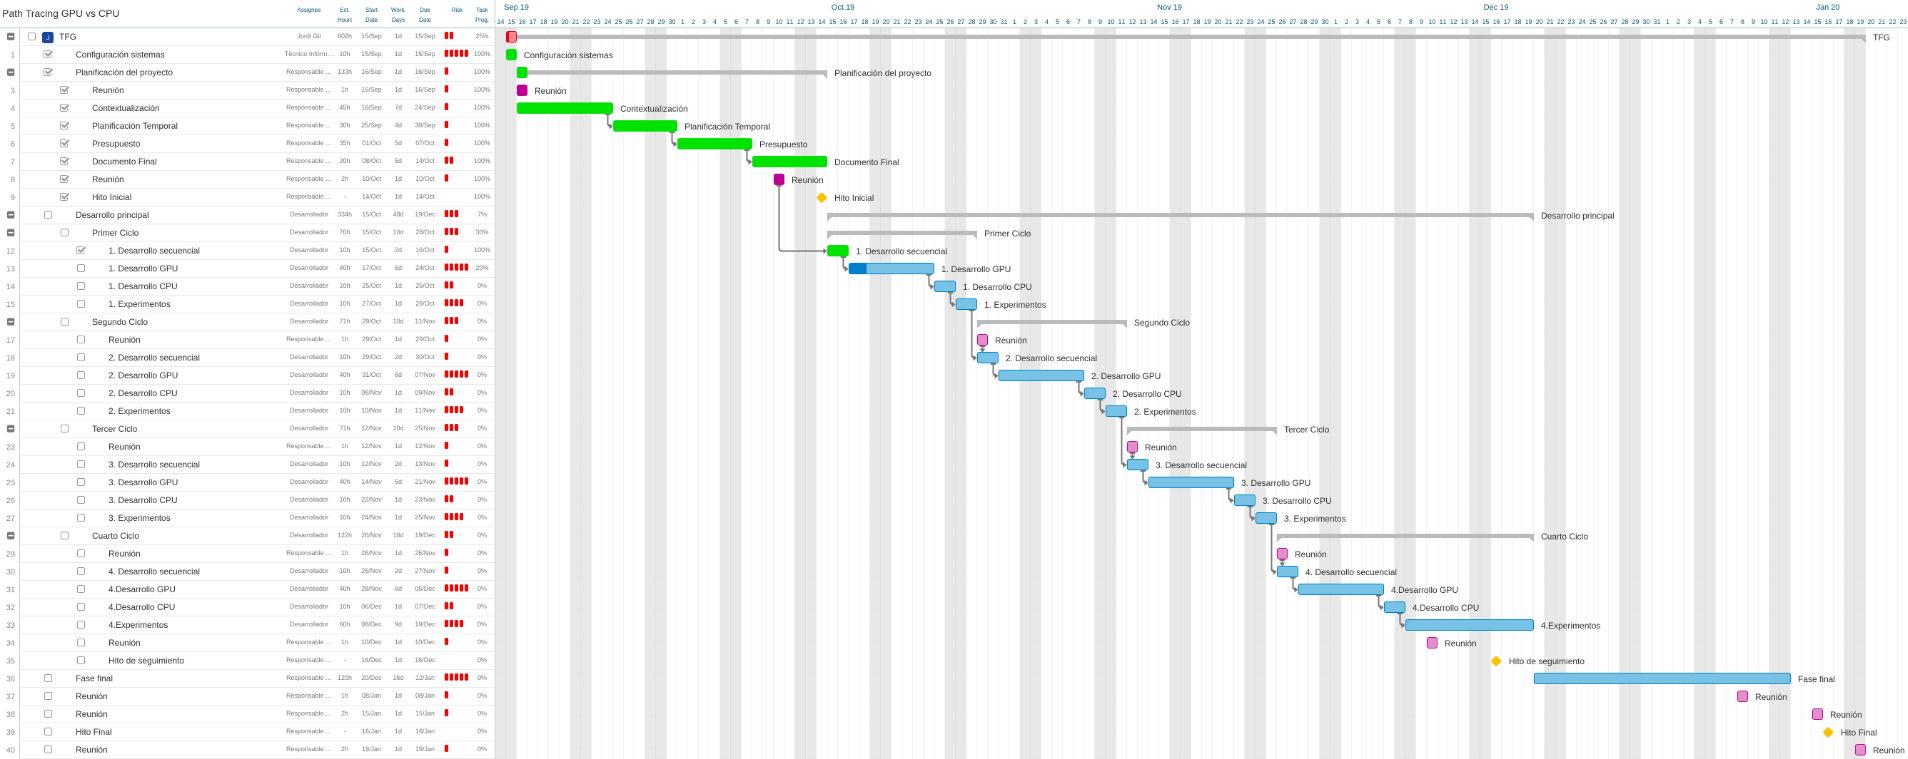
\includegraphics[scale=1.45]{media/final_gantt.png}
	\captionof{figure}{Diagrama de Gantt completo.}
	\label{gantt}
\end{figure}

\begin{figure}[H]
	\centering
  	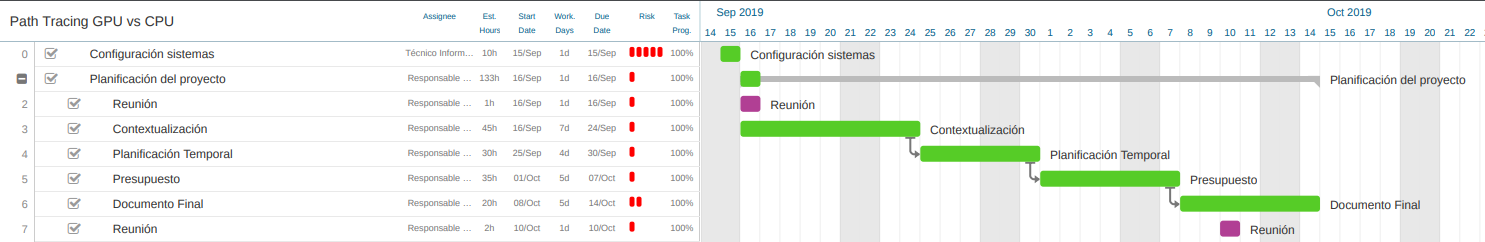
\includegraphics[scale=1.5]{media/final_gantt_1.png}
  	\captionof{figure}{Etapa de gestión.}
  	\label{gantt_1}
\end{figure}

\begin{figure}[H]
	\centering
  	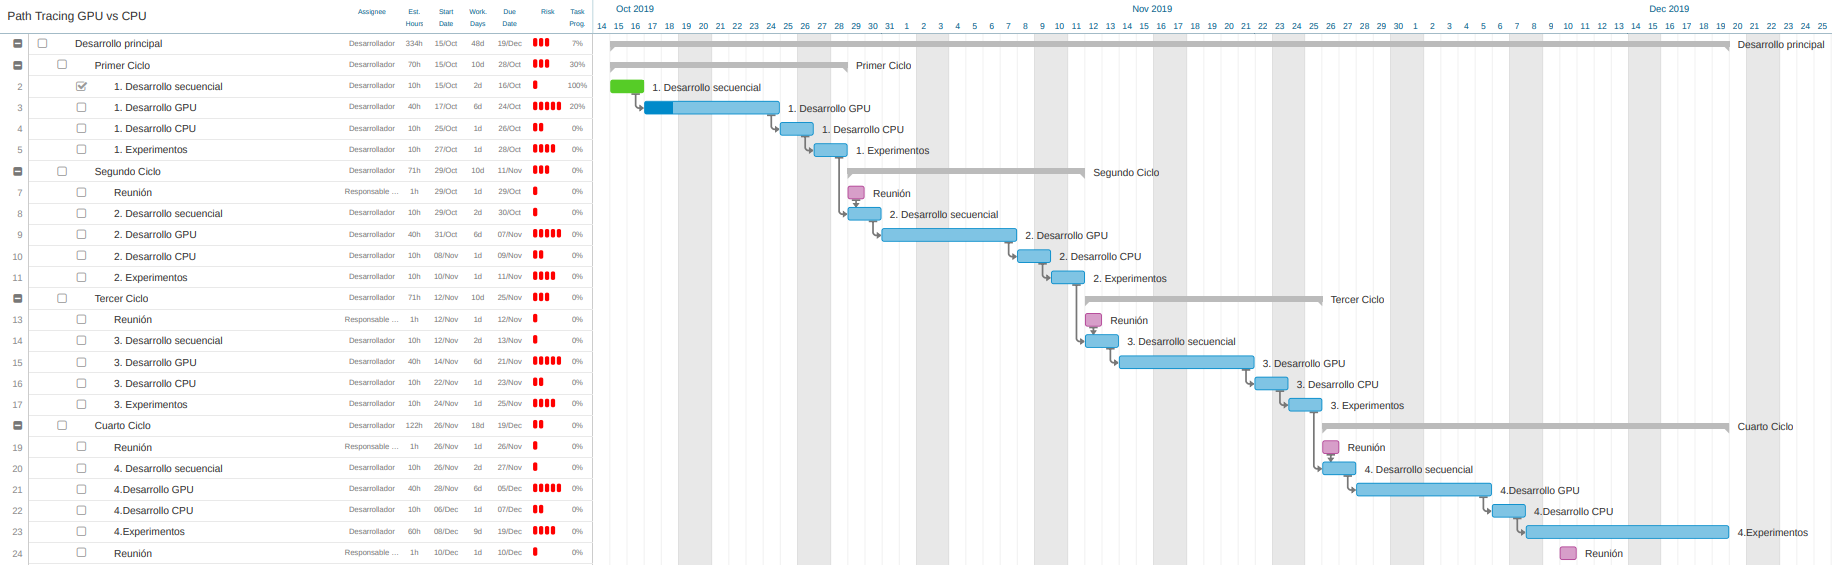
\includegraphics[scale=1.25]{media/final_gantt_2.png}
  	\captionof{figure}{Etapa de desarrollo.}
  	\label{gantt_2}
\end{figure}

\useportrait

\chapter{Presupuesto y sostenibilidad}

En este capítulo trataremos los temas de presupuesto y sostenibilidad. Veremos una descripción detallada de los costes del proyecto, de los recursos tanto materiales como humanos, y un análisis de cómo podrían afectar a nuestro presupuesto los diferentes obstáculos que pueden acaecer en el trascurso del desarrollo. Haremos también una evaluación de la sostenibilidad del proyecto.

El presupuesto puede estar sujeto a modificaciones a lo largo del desarrollo del proyecto.

\section{Presupuesto}

En esta sección veremos como hacer una estimación del presupuesto por tal de poder desarrollar el proyecto. Podemos dividir el presupuesto en dos grandes secciones: \begin{enumerate*}[label=\roman*)] \item Costes directos y \item Costes indirectos
\end{enumerate*}.

\subsection{Costes directos}

Los costes directos los dividiremos en función de los diferentes tipos de recursos que tenemos en este proyecto: \begin{enumerate*}[label=\roman*)] \item software, \item hardware y \item humanos \end{enumerate*}.

Para el cálculo de la amortización tendremos en consideración que el proyecto tiene una duración aproximada de cinco meses.

\subsubsection{Recursos de Software}

El software que vamos a utilizar en nuestro proyecto es de código libre, por lo tanto se trata de software gratuito. En caso de necesitar software adicional intentaremos que este sea también de código libre. La Tabla \ref{soft} muestra el coste del software utilizado en el desarrollo.

\begin{table}[H]
	\centering
	\begin{tabular}{|c|c|c|c|}
		\hline
		\textbf{Producto} & \textbf{Precio} & \textbf{Vida útil} & \textbf{Amortización} \\ \hline \hline
		Ubuntu 18.04 	& 0,00€ & - & 0,00€ \\ \hline
		\LaTeX\ 		& 0,00€ & - & 0,00€ \\ \hline
		CUDA 			& 0,00€ & - & 0,00€ \\ \hline
		OpenMP 			& 0,00€ & - & 0,00€ \\ \hline
		C++ 			& 0,00€ & - & 0,00€ \\ \hline	\hline
		Total 			& 0,00€ & - & 0,00€ \\ \hline
	\end{tabular}
	\caption{Coste recursos de software}
	\label{soft}
\end{table}

\subsubsection{Recursos de Hardware}

La Tabla \ref{hard} muestra el coste del hardware utilizado en el desarrollo. En la amortización se tiene en cuenta una duración aproximada de cinco meses de proyecto como bien hemos especificado al inicio de esta sección. Si aproximadamente un año tiene 365 días y la vida útil de las máquinas utilizada son de 5 años, esto nos da un total de 1825 días de vida útil. El proyecto dura de septiembre a enero, ambos incluidos, por lo tanto la duración es de 153 días.

\begin{table}[H]
	\centering
	\resizebox{\textwidth}{!}{\begin{tabular}{|c|c|c|c|c|}
		\hline
		\textbf{Producto} 	& \textbf{Precio} & \textbf{Vida útil (en años)} & \textbf{Amortización/día} & \textbf{Amortización} \\ \hline \hline
		PC Sobremesa 		& 2210,09€ & 5 & 1,21€/día & 185,13€\\ \hline
		Lenovo Legion Y520 	&  900,00€ & 5 & 0,49€/día &  74,97€ \\ \hline
		BOADA 				& 3500.00€ & 5 & 1,92€/día & 293,76€ \\ \hline \hline	
		Total 				& 6610.09€ & - & -         & 553,86€ \\ \hline
	\end{tabular}}
	\caption{Coste recursos de hardware}
	\label{hard}
\end{table}

En el coste del cluster de docencia, BOADA, no se tienen presente las cuatro tarjetas gráficas NVIDIA Tesla K40c puesto que fueron una donación de \textit{NVIDIA}, por lo que su coste es nulo.

\subsubsection{Recursos Humanos}

Para cada tarea especificada en el GANTT, Figure \ref{gantt}, le identificaremos el rol más adecuado, como podemos ver listados a continuación:

\begin{itemize}
	\item \textbf{Responsable del proyecto:} Planificación del proyecto, fase final y reuniones con el director del proyecto.
	\item \textbf{Desarrollador de software:} Desarrollo de las tres aplicaciones y experimentos.
	\item \textbf{Técnico informático:} Configuración del sistema.
\end{itemize}

En la Tabla \ref{rrhh_0} podemos visualizar las tareas asignadas a cada rol y el número de horas estimadas.

\begin{table}[H]
	\centering
	\begin{tabular}{|c|c|c|}
		\hline
		\textbf{Categoría} & \textbf{Tarea} & \textbf{Horas} \\ \hline \hline
		Director de proyecto 	  & Reuniones/correos 			&  92h \\ \hline
		Responsable de proyecto   & Planificación del proyecto	& 130h \\ \hline
		Responsable de proyecto   & Etapa final					& 120h \\ \hline
		Responsable de proyecto   & Reuniones					&  12h \\ \hline
		Desarrollador de software & Desarrollo   		 		& 240h \\ \hline
		Desarrollador de software & Experimentos				&  90h \\ \hline
		Técnico informático 	  & Configuración del sistema	&  10h \\ \hline
	\end{tabular}
	\caption{Relación rol - tareas.}
	\label{rrhh_0}
\end{table}

En la Tabla \ref{rrhh_1} podemos observar la relación del salario en €/hora y el número de horas trabajadas por cada uno de los roles. 

Para determinar el sueldo de cada rol se ha consultado el portal web \citep{tuSalario} teniendo en cuenta el propio rol y realizando una aproximación de la experiencia de la persona que lo desempeña en el proyecto (por ejemplo la experiencia que pueda tener el director del proyecto, desempeñado por un profesor senior o la experiencia como desarrollador de un estudiante que finaliza los estudios de un grado universitario) y aplicando el coste a la Seguridad Social (aproximadamente el salario bruto multiplicado por 1,35).

\begin{table}[H]
	\centering
	\resizebox{\textwidth}{!}{\begin{tabular}{|c|c|c|c|c|}
		\hline
		\textbf{Categoría} & \textbf{Salario bruto €/h} & \textbf{Salario bruto €/h + SS} & \textbf{Horas Totales} & \textbf{Coste estimado} \\ \hline \hline
		Director de proyecto 	  & 18€/h & 24,30€/h &  92h & 2235,60€ \\ \hline
		Responsable de proyecto   & 15€/h & 20,25€/h & 262h & 5305,50€ \\ \hline
		Desarrollador de software & 13€/h & 17,55€/h & 330h & 5791,50€ \\ \hline
		Técnico informático 	  & 11€/h & 14,85€/h &  10h &  148,50€ \\ \hline \hline			
		Total 					  & - 	  & - 		 & 694h & 13481,10€ \\ \hline
	\end{tabular}}
	\caption{Coste recursos de RRHH}
	\label{rrhh_1}
\end{table}

\subsection{Costes indirectos}

En esta sección tendremos en cuenta los costes que se relacionan con el proyecto de forma indirecta, como el derivado del consumo energético y el coste de la red de Internet.

Teniendo presente las diferentes máquinas que se utilizan en el proyecto el consumo de cada una de ellas es el siguiente:

\begin{enumerate}
	\item \textbf{PC Sobremesa:} 320W.
	\item \textbf{Lenovo Legion Y520:} 160W.
	\item \textbf{Cluster docencia BOADA:} 1500W.
\end{enumerate}

A continuación, en la Tabla \ref{ci_1} podemos observar la relación entre las tareas realizadas y la máquina utilizada en cada una de ellas.

\begin{table}[H]
	\centering
	\resizebox{\textwidth}{!}{\begin{tabular}{|c|c|c|c|c|c|c|}
	\hline
	\multirow{2}{*}{\textbf{Máquina}} & \multicolumn{5}{c|}{\textbf{Tareas}} & \textbf{Coste} \\ \cline{2-6} 
			& Configuración & Planificación & Desarrollo & Experimentos & Fase final & \textbf{Estimado} \\ \hline \hline
		PC Sobremesa 			& 5h  & 130h & 240h & 30h &	120h & 525h \\ \hline
		Lenovo Legion Y520 		& 5h  & -	 & -    & 30h &	-	 & 35h\\ \hline
		BOADA 					& -	  & -	 & -    & 30h &	-	 & 30h\\ \hline
	\end{tabular}}
	\caption{Horas por tarea y recurso}
	\label{ci_1}
\end{table}

Para determinar el coste del kW por hora hemos consultado el portal \citep{tuLuz}, calculando la media del precio entre las diferentes compañías eléctricas mostradas. 

En la Tabla \ref{ci2} podemos observar el coste de la energía consumida por cada una de las máquinas en función del número de horas en que utilizamos dichas máquinas en las diferentes tareas del proyecto. En \textit{generales} se contemplan costes como: \begin{enumerate*}[label=\roman*)] \item compra de material (papel, bolígrafos, etc) y \item transporte (desplazamiento para reuniones, etc). \end{enumerate*}. 

\begin{table}[H]
	\centering
	\begin{tabular}{|c|c|c|c|}
		\hline
		\textbf{Máquina} & \textbf{Precio} & \textbf{Unidades} & \textbf{Coste estimado} \\ \hline \hline
		PC Sobremesa 			& 0,13508€/kWh & 168kWh 	&  22,39€ 	\\ \hline
		Lenovo Legion Y520 		& 0,13508€/kWh & 5,6kWh 	&   0,76€ 	\\ \hline
		BOADA 					& 0,13508€/kWh & 45kWh 		&   6,08€ 	\\ \hline 
		Internet				& 50€		   & 6 meses	& 300,00€ 	\\ \hline
		Generales 				& 120€ 		   & -          & 120,00€	\\ \hline \hline
		Total 					& - 		   & -			& 449,23€	\\ \hline
	\end{tabular}
	\caption{Coste de consumo por máquina}
	\label{ci2}
\end{table}

\subsection{Costes inesperados}

En caso de alguna desviación en la planificación del proyecto, destinaremos una parte del presupuesto a los contratiempos que puedan surgir.

\begin{table}[H]
	\centering
	\resizebox{\textwidth}{!}{\begin{tabular}{|c|c|c|c|c|}
		\hline
		\textbf{Categoría} & \textbf{Salario neto €/h} & \textbf{Salario bruto €/h} & \textbf{Horas Totales} & \textbf{Coste estimado} \\ \hline \hline
		Director de proyecto 	  & 18€/h & 24,30€/h & 20h  &  486,00€  \\ \hline
		Responsable de proyecto   & 15€/h & 20,25€/h & 10h  &  202,50€  \\ \hline
		Desarrollador de software & 13€/h & 17,55€/h & 20h  &  351,00€  \\ \hline
		Técnico informático 	  & 11€/h & 14,85€/h &  2h  &   29,70€  \\ \hline \hline			
		Total 					  & - 	  & - 		 & -    & 1069,20€  \\ \hline
	\end{tabular}}
	\caption{Costes inesperados}
	\label{rrhh_2}
\end{table}

\subsection{Presupuesto total}

En la Tabla \ref{total} podemos observar el presupuesto total del proyecto completo y con una contingencia de un 10\% por posibles improvistos.

\begin{table}[H]
	\centering
	\begin{tabular}{|c|c|}
		\hline
		\textbf{Concepto} 		& \textbf{Coste estimado} \\ \hline \hline
		\multicolumn{2}{|c|}{Coste directo}  	\\ \hline
		Software 				&     00,00€  	\\
		Hardware				&    553,86€  	\\ 
		RRHH 					&  13481,10€  	\\ \hline 
		Coste indirecto			&    449,23€  	\\ \hline
		Coste inesperado		&   1069,20€	\\ \hline		
		\textbf{Subtotal}		&  15553,39€  	\\ \hline
		Contingencia (10$\%$) 	&   1555,34€  	\\ \hline \hline
		\textbf{Total}			&  17108,73€  	\\ \hline
	\end{tabular}
	\caption{Presupuesto total}
	\label{total}
\end{table}

\section{Control de gestión}

En lo referente a los recursos humanos, al no tratarse de una inversión inicial no puede realizarse un control constante. Solamente podremos comparar el coste final con el presupuestado una vez el proyecto haya finalizado.

En cuanto a los recursos materiales y digitales (software) sí podemos y debemos realizar un control constante. Con tal de realizar un control presupuestario, al final de cada una de las tareas haremos un recuento de las horas empleadas y el coste del material extra utilizado, si se diera el caso. Con esta información podremos hacer una comparativa con los datos estimados previamente y calcular la desviación. En caso de realizarse un desvío importante se deberá realizar un estudio con tal de esclarecer el porqué del desvío y corregir las estimaciones del presupuesto en las siguientes tareas o fases del proyecto a realizar.

Si una vez finalizado el proyecto, la suma de las diferencias en todas las fases nos indica una incorrecta previsión presupuestaria, es decir, nos hemos quedado cortos en el presupuesto inicial propuesto, entonces deberemos asignar el fondo de contingencia en cubrir los gastos extras ocasionados.

Por tal de calcular las desviaciones, utilizaremos las fórmulas siguientes:

\begin{itemize}

	\item Desvío de mano de obra en precio = (coste std - coste real) * consumo de horas real.
	\item Desvío de un recurso en precio = (coste std - coste real) * consumo real.
	\item Desvío de mano de obra en consumo = (consumo horas std - consumo horas reales) * coste std.
	\item Desvío de un recurso en consumo = (consumo estimado - consumo real) * coste real.
	\item Desvío total en mano de obra = total coste std mano de obra - total coste real mano de obra.
	\item Desvío total en recursos = total coste std recursos - total coste real recursos.

\end{itemize}

\section{Sostenibilidad}

\subsection{Autoevaluación}

En la encuesta diseñada por los miembros del proyecto EDINSOST se nos realizan una serie de preguntas con el fin de auto evaluar nuestro conocimiento en materia de sostenibilidad.

Realizando la encuesta, he podido observar que carezco de análisis en materia de sostenibilidad a la hora de realizar cualquier tipo de proyecto. Soy capaz de reconocer las causas y consecuencias que pueden presentarse pero no de las posibles soluciones que existen al respecto. Pocas son las veces que he analizado un proyecto o problema desde el punto de vista de la sostenibilidad.

Si bien como he comentado soy capaz de reconocer las consecuencias ambientales y sociales que un proyecto pueda tener, al no tener en cuentas estos efectos no sé bien como medir el impacto real que puedan tener. Al no conocer que herramientas o métricas se utilizan comúnmente para analizar el impacto de un proyecto en estos tres ámbitos, podría ser que estuviera repercutiendo de forma negativa en ellos.

En general, al no ponerme a analizar un problema desde este punto de vista, el de la sostenibilidad, soy incapaz de comprender que efectos sociales, ambientales y económicos pueden haber.

A pesar de comprender la necesidad de introducir justicia social, equidad, transparencia, etc. en un proyecto, a día de hoy no estoy poniendo en práctica estas necesidades por lo que tengo poca idea o soy incapaz de estimar el impacto real que un proyecto pueda acontecer a la sociedad. Y si este contribuye o no al bien común.
Sé valorar la viabilidad económica de un proyecto, pero no de compatibilizarla con los ámbitos: ambiental y social.

En proyectos colaborativos, conozco y utilizo herramientas que facilitan el trabajo entre los diferentes integrantes y valoro positivamente el trabajo realizado por los demás.

En conclusión, a pesar de conocer las causas y consecuencias que un proyecto podría tener en los ámbitos: ambiental, económico y social, esta encuesta me ha permitido ver que existe una dejadez en mí en cuanto al análisis de estas consecuencias. Necesito informarme y concienciarme más respecto a estos temas para poder aplicarlos en futuros proyectos.

\subsection{Impacto ambiental}

El impacto ambiental producido por el presente proyecto no es más que el resultado del consumo de electricidad por parte de las máquinas que utilizamos. Al tratarse de un proyecto experimental sobre un algoritmo en concreto, no estamos creando ningún tipo de producto físico por lo que no se ha planteado el uso de material reciclado o material de proyectos similares anteriores.

En la Tabla \ref{rrhh_1} podemos observar que el total de horas que concierne a los recursos humanos son de 670h. Considerando que una persona en su rutina habitual tiene un consumo de 0,1kWh, el consumo total es de $0,1kWh \cdot 670h = 67kWh$.

Como hemos comentado en la sección anterior, utilizamos tres máquinas diferentes para realizar los experimentos, pero para el desarrollo íntegro del proyecto solamente estamos utilizando una de ellas. El proyecto se realiza en la máquina que tiene un consumo de 250W, teniendo en cuenta las horas utilizadas por esta máquina, según vemos en la Tabla \ref{ci_1}, el consumo total es de $0,25kWh \cdot 525h = 131,25kWh$. Si bien es cierto que no se analizó el impacto ambiental que el presente proyecto pudiera tener para así poder minimizarlo, ahora, teniendo una mayor perspectiva podríamos haber optado por realizar el proyecto en la máquina de menor consumo energético y remitir las otras solamente a los experimentos (que requieren menos horas de trabajo y por ende un menor consumo energético).

Según la Generalitat de Catalunya \citep{gene}, el año 2018 se estima que la emisión de $CO_{2}$ por parte de la red eléctrica peninsular era de 321g $CO_{2}/kWh$. En nuestro proyecto estamos consumiendo un total de 218kWh, esto supone una emisión de 69,978kg de $CO_{2}$ a la atmósfera. Un vuelo Barcelona -  Nueva York son 1.177 kilogramos según \citep{hostel}. Nuestro proyecto emite casi un 6\% de las emisiones de $CO_{2}$ de un vuelo comercial Barcelona - Nueva York.

Por último, cabe mencionar que el presente proyecto no ofrece ningún tipo de mejora ambiental respecto a proyecto/productos similares. El impacto ambiental que pueda suponer el consumo de electricidad depende exclusivamente del suministrador y no tiene el mismo impacto el uso de energías renovables que el uso de energías fósiles.

\subsection{Impacto económico}

Todos los costes relativos al presente proyecto han sido detallados en la sección anterior de los recursos utilizados, tanto humanos como de software y hardware. A pesar de haber varios roles definidos, estos serán llevados por una sola persona (a excepción del rol de "Director del proyecto"). Esto supone que el coste humano se reduce a solamente dos personas. 

El principal coste económico que observamos en el proyecto es el de hardware. Éste podría reducirse haciendo, quizás, un menor uso de máquinas, pero limitando así los objetivos del proyecto. Es por eso que creemos que el gasto económico es el adecuado.

\subsection{Impacto social}

A título personal, este proyecto me permite adquirir nuevos conocimientos no vistos a lo largo del grado y definir también los pasos a seguir en el futuro, ayudándome a guiar mi futuro profesional y/o académico.

Una vez finalizado el proyecto no tendrá gran trascendencia en la sociedad en general. Como comentamos en capítulos anteriores, este proyecto no propone ninguna alternativa respecto a soluciones existentes sino más bien dar una serie de herramientas al autor de éste para adentrarse en el mundo de la computación gráfica realista. Por lo tanto, es difícil de determinar el impacto social que pueda tener más allá del divulgativo o académico.

\newpage

\printbibliography

\listoffigures

\listoftables

\end{document}
